\documentclass[twocolumn]{article}
\usepackage[UTF8]{ctex}    % 中文语言包
%\usepackage{multicol}  % 用于实现在同一页中实现不同的分栏
\usepackage[shortlabels]{enumitem}    % 编号扩展功能包
\usepackage{graphicx}    % 图片功能包
\usepackage{subfigure}    % 子图功能包
\usepackage{booktabs}    % 表格功能包
\usepackage{multirow}    % 合并多行表格
\usepackage{amsmath}    % 公式功能包
\usepackage{amsfonts, amssymb}  % 空心字母
\usepackage{cuted}        % 公式跨栏表示 
\usepackage{minted}     % 代码高亮
\setminted{fontsize=\footnotesize}{\normalsize {\tiny {\scriptsize {\footnotesize }}}}
\newcommand{\upcite}[1]{\textsuperscript{\textsuperscript{\cite{#1}}}}  % 参考文献设置在右上角
%\usepackage{stfloats}

% 伪代码的格式设置
%%***************************************************************************************************
%% 头文件部分
%\makeatletter
%\newif\if@restonecol
%\makeatother
%\let\algorithm\relax
%\let\endalgorithm\relax
%\usepackage[linesnumbered,ruled,vlined]{algorithm2e}%[ruled,vlined]{
%\usepackage{algpseudocode}
%\renewcommand{\algorithmicrequire}{\textbf{Input:}}  % Use Input in the format of Algorithm
%\renewcommand{\algorithmicensure}{\textbf{Output:}} % Use Output in the format of Algorithm 
%%***************************************************************************************************



\usepackage{algorithm}
\usepackage{algorithmicx}
\usepackage{algpseudocode}

\floatname{algorithm}{算法}
\renewcommand{\algorithmicrequire}{\textbf{输入:}}
\renewcommand{\algorithmicensure}{\textbf{输出:}}



\usepackage{titlesec}  % 自定义多级标题格式的宏包

% \titleformat{command}[shape]  % 定义标题类型和标题样式,字体
% {format}  % 定义标题格式:字号(大小),加粗,斜体 例如 \fontsize{20.75pt}\bfseries\centering
% {label}  % 定义标题的标签,即标题的标号等
% {sep}  % 定义标题和标号之间的水平距离
% {before-code}  % 定义标题前的内容

\titleformat{\section}[block]%定义标题类型和标题样式,字体
{\Large\bfseries}  % 定义标题格式:字号(大小),加粗(,斜体),居中
{\bfseries\arabic{section}}  % 定义标题的标签,即标题的标号等
{0.5em}  % 定义标题和标号之间的水平距离
{}  % 定义标题前的内容
[]  % 定义标题后的内容

\titleformat{\subsection}[block]  % 定义标题类型和标题样式,字体
{\large\bfseries}  % 定义标题格式:字号(大小),加粗,斜体
{\bfseries\arabic{section}.\bfseries\arabic{subsection}}  % 定义标题的标签,即标题的标号等
{0.5em}  % 定义标题和标号之间的水平距离
{}  % 定义标题前的内容
[]  % 定义标题后的内容

\titleformat{\subsubsection}[block]  % 定义标题类型和标题样式,字体
{\normalsize\bfseries}  % 定义标题格式:字号(大小),加粗,斜体
{\bfseries\arabic{section}.\bfseries\arabic{subsection}.\bfseries\arabic{subsubsection}}  % 定义标题的标签,即标题的标号等
{0.5em}  % 定义标题和标号之间的水平距离
{}  % 定义标题前的内容
[]  % 定义标题后的内容

\titleformat{\paragraph}[block]
{\small\bfseries}
{[\arabic{paragraph}]}
{1em}
{}
[] 

% \titleformat{\section}[block]{\LARGE\bfseries}{\Roman{section}}{1em}{Hello: }[]
% \titleformat{\subsection}[block]{\Large\itshape\mdseries}{\arabic{section}.\arabic{subsection}}{0.5em}{}[]
% \titleformat{\subsubsection}[block]{\normalsize\bfseries}{\arabic{subsection}-\arabic{subsubsection}}{0em}{}[]
% \titleformat{\paragraph}[block]{\small\bfseries}{[\arabic{paragraph}]}{1em}{}[]



\usepackage{setspace}  % 设置行间距
\usepackage{geometry}  % 设置一些页面格式,还没开发安全
\geometry{a4paper,left=2.0cm,right=2.0cm,top=2.25cm,bottom=2.0cm}

% 正文字体的设置
\PassOptionsToPackage{no-math}{fontspec}
\usepackage{mathspec}
\setmainfont{Times New Roman}  % 正文英文字体的设置
\setCJKmainfont{SimSun}[AutoFakeBold,ItalicFont=KaiTi]  % 正文中文字体的设置
\setCJKsansfont{SimHei}%对应sf无衬线
\setCJKmonofont{FangSong}%对应tt打字机
%\newCJKfontfamily{\kaishu}[AutoFakeBold={2.17}]{STXingkai}


% 摘要格式的设置
\usepackage{tikz}
\usetikzlibrary{shapes,shadows}
\tikzstyle{abstractbox} = [draw=black, fill=white, rectangle, 
inner sep=20pt, style=rounded corners, drop shadow={fill=black,
	opacity=0.5}]
\tikzstyle{abstracttitle} =[fill=white]

\newcommand{\boxabstract}[2][fill=white]{
	\begin{center}
		\begin{tikzpicture}
			\node [abstractbox, #1] (box)
			{\begin{minipage}{0.82\linewidth}
					\setlength{\parindent}{2mm}
					\small #2
			\end{minipage}};
			\node[abstracttitle, right=10pt] at (box.north west) {\textbf{摘要}};
		\end{tikzpicture}
	\end{center}
}
	
	
%\newsavebox{\myabstractbox}
%\providecommand{\abstractnode}[2]{
	%	\begin{tikzpicture}%
		%		\node [abstractbox, fill=#1](box)%
		%		{#2};%
		%		\node[abstracttitle, right=10pt] at (box.north west) {Abstract};
		%	\end{tikzpicture}
	%}
%
%
%\newenvironment{abstractbox][1][white]{
%		\begin{center}%
	%			\def\abs@bgcok{#1}%
	%			\begin{Irbox}{\myabstractbox}
		%				\begin{minipage}{.80\linewidth}%% lparindent2em%
			%					\footnotesize #2
			%				\end{minipage}
		%			\end{Irbox}
	%%			\abstractnode{\abs@bgcol}{\usebox{\myabstractbox}}%
	%		\end{center}%
%	}
		
\makeatletter
\newenvironment{tablehere}
{\def\@captype{table}}
{}

\newenvironment{figurehere}
{\def\@captype{figure}}
{}
\makeatother
		


%opening
\title{嵌入空间中的主题建模(Topic Modeling in Embedding Spaces)}
\author{{\small 周方全\footnote{电子科技大学计算机科学与工程学院2021级计算机科学与技术专业 \quad \textbf{学号}: 202121081229 \quad \textbf{邮箱地址}: 2542154447@qq.com} \quad\quad 研究方向:自然语言处理} }
\date{}


{\tiny {\small }}
\begin{document}
\maketitle  % 生成标题

%\begin{abstractbox}
%    {\bf \rm} \newline    \newline    
%    {\bf\emph{ Key words-\ 语义切割; ; }\rm}    % 文字直接在创建好的环境中输入就可以了。编译后就可以看到效果。
%\end{abstractbox}
\boxabstract{    
%    \kaishu
    {   本文的主要工作是复现了一篇来自ACL的文章\cite{dieng2020topic}。这篇文章
        提出了embedded topic model(ETM),这是一种将传统的主题模型嫁接到词向量空
        间中的文本生成模型。同时,为了训练ETM,\cite{dieng2020topic}提出了一个高
        效的变分推断算法。ETM在保留停用词和低频词的情况下依然能够获得很好的可解释
        性主题。本文首先介绍ETM模型,然后介绍变分自动编码器及其中的数学推导过程,
        最后展示实验的复现结果。
        \rm} \newline    \newline    
    {   \textbf{关键词\quad}  主题模型, ETM, 变分自动编码器, 词向量空间 \rm}
}
%\begin{multicols}{2}  
\section{介绍}
	$\mathbb{1}$
    主题模型是用于发现文档集合中隐藏的语义结构的统计工具。主题模型及其扩展已经应用
    于许多领域,如市场营销、社会学、政治科学和数字人文学科等。其中大多数的主题模型
    都是在latent Dirichlet allocation(LDA)\cite{blei2003latent}的基础上建立起来的。LDA是一个层次化
    的概率模型,它将每个主题表示为按术语分布的分布,并将每个文档表示为主题的混合体。
    但是LDA在处理大型文档的时候效果很差。之前也有人通过删减文档高频词和低频词来削减
    文档的词汇量,但是这样做可能会删掉文档中的重要词汇。而且,LDA是基于词袋的一种模型,
    这样做会丢失单词与单词之间的语义联系。
    
    面对这两个问题,ETM都比LDA具有先天性的优势。
    首先,ETM是基于word embedding的模型。word embedding是一种将单词嵌入到词向量的表示
    方法,意思相近的两个单词的词向量的余弦值更大。其次,ETM在处理文档的时候不需要去除停用词
    和低频词。如图\ref{fig:001}我们可以直观地看到两个模型在面对文档词汇量逐渐增大的时候,生成主题的
    效果。Coherence-Normalized Perplexity是一种描述生成主题好坏的量化指标。
\begin{figure}
    \centering
    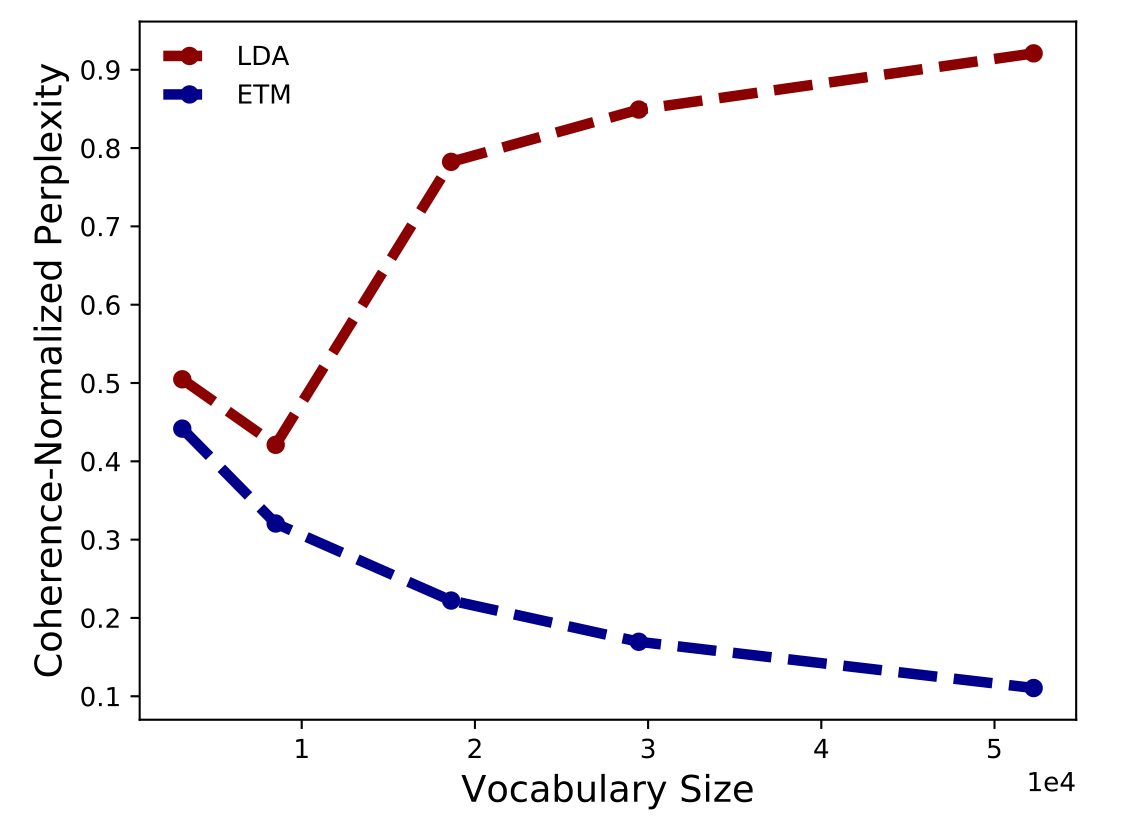
\includegraphics[width=0.7    \linewidth]{figures/001}
    \caption{{\small 两种模型在面对文档词汇量增大时的效果对比}}
    \label{fig:001}
\end{figure}

    和LDA相似的是,ETM也是一个生成概率模型。对于每一个文档都有一个主题分布,而对于没有个主题
    都有一个词汇分布,我们的主题的选择是在所有词汇中间选取的。面对一个具体的文档和其主体
    分布,加入我们要选择20个主题。我们就选择概率最高的这二十个主题。而每个主题都有一个单词分布,
    同样是对应概率高的词汇越有机会是该主题。


\section{ETM模型详解}
    ETM模型是LDA和词向量模型结合版。它主要运用了LDA的思想,并将参数的训练放到了一个变分自编码器上。
    在介绍模型之前我们先说明一些符号和其意思。假设我们有一个含有$ D $个文档的语料库$ \{{{\bf{w}}_1},...,{{\bf{w}}_d},...,{{\bf{w}}_D}\} $,这个语料库含
    有$ V $个互不相同的单词——词库。$ w_{dn} \in \{1,...,V\}$表示第$ d^{th} $个文档的第
    $ n^{th} $个单词。每个文档有$ K $ 个主题,$ \varphi_i $表示第$ i $个主题,其中$ i \in (1, K) $。
    
\subsection{LDA文本生成过程}
    LDA认为,一个文档除了能够观察到的词以外还有无法被观测到的主题,而其生成过程是给定一篇文档,当需要生成一个词的时候先确定生成的词的主题,然后根据指定的主题再生成相应的词。当然,一篇文档会有多个主题,这时候多个主题就形成了一个概率分布,每生成一个词的时候就根据这个分布采样,获得当前词的主题。获得了一个主题后,需要生成合适的词,而和一个主题相关的词同样有很多。在不同的主题下,同一个词有不同的被选择的概率,当然,同一主题下,不同的词存在不同的被选择的概率。这时,词汇库里面的词就形成了一个概率分布。在LDA中,主题分布和词汇分布都是类别分布,分别用符号 $ \theta $ 和 $ \varphi $表示。此外,LDA需要预先确定主题的数量,一般用 $ K $ 表示。前面我们说过,不同的主题有着不同的词汇分布,所以一共有$ K $ 个词汇分布,分别用 $ \varphi_i, \{i \in (1, K)\} $ 表示,与第$ i $个主题相对应。以上是LDA生成一篇文档的主要思想。
    
    大多数情况下,我们拥有的是一个文档集。同样很自然的,不同的文档主题会有差异,所以其对应的主题分布$ \theta $ 也会不同,与主题的词汇分布类似,LDA认为不同的文档对应的主题分布是不同的,所以对于文档$ d $来说,其主题分布可以用$ \theta_d $表示。从频率学派的角度来看,文档的建模已经完成了,但是对于贝叶斯学派来说,模型的参数不是一个确定的值,所以需要对上面的参数进行建模,而上面属于模型的参数是主题分布$ \theta $和词汇分布$ \varphi $。LDA则从贝叶斯角度出发,假设这两个参数符合狄利克雷分布,表示为 $ \theta \sim Dir(\alpha)$ ,$\varphi \sim Dir(\beta)$。所以,在LDA的假设下,每个文档集的生成可以表示为如下形式:
\begin{enumerate}[I.]
    \item 确定文档数$ D $,主题数$ K $,词汇库大小$ V $,预设参数$ \alpha = (\alpha_1,...,\alpha_d,...,\alpha_D) $和$ \beta = (\beta_1,...,\beta_k,...,\beta_K) $
    \item 生成$ K $个主题的词汇分布$ \varphi = \{\varphi_1,...,\varphi_k,...,\varphi_K\} $,$ \varphi \sim Dir(\beta) $
    \item 对文档$ {{\bf{w}}_d} $:
           \begin{enumerate}[i.]
                  \item 生成文档的主题分布$ \theta_d \sim Dir(\alpha) $
                  \item 对文档$ {{\bf{w}}_d} $中的每个词$ w_{dn} $:
                          \begin{enumerate}[a.]
                              \item 生成其主题$ z_n \sim cat(\theta_d) $
                              \item 生成词$ w_{dn} \sim cat(\varphi_{z_n}) $
                          \end{enumerate}
          \end{enumerate}
\end{enumerate}
从上面我们可以发现,LDA的效果受预设的主题数$ K $ ,以及预设参数 $ \alpha $ 和 $ \beta $ 的影响。

\subsection{ETM文本生成过程}
    在ETM中词是用词向量表示的,而不是用LDA所使用的词袋。所以,我们需要定义一个词向量矩阵
    $ \rho \in \Re^{L \times V}$。同样,将$ K $个主题定义成$ K $个长度为L的向量$ \alpha_k \in \Re^L $
    ,此时主题和词处于同一个语义空间。
    
    在ETM模型下,文档生成过程和LDA没有区别,依然需要使用文档的主题分布$ \theta $以及主题的词汇分布$ \varphi $,只是具体采用的分布和训练的过程发生了变化。在ETM中这两个参数的分布分别采用了,$ \theta \sim \mathcal{LN}(0, I) \Leftrightarrow \delta \sim \mathcal{N}(0, I)$ , $\theta = softmax(\delta)$ ;$ \varphi \sim softmax(\rho^\top \alpha_k) $ 。也就是说,文档的主题分布是一个多维对数标准正态分布,而主题的词汇分布则是主题的向量表示与各个词的词向量点乘后的softmax后的结果。文本的生成过程则变为:
\begin{enumerate}[I.]
    \item 确定文档数$ D $,主题数$ K $,词汇库大小$ V $
    \item 对文档$ {{\bf{w}}_d} $:
    \begin{enumerate}[i.]
        \item 生成文档的主题分布$ \theta_d = softmax(\delta_d) $,$ \delta_d \sim \mathcal{N}(0, I) $
        \item 对文档$ {{\bf{w}}_d} $中的每个词$ w_{dn} $:
        \begin{enumerate}[a.]
            \item 生成其主题$ z_n \sim cat(\theta_d) $
            \item 生成词$ w_{dn} \sim softmax(\rho^\top \alpha_{zn}) $
        \end{enumerate}
    \end{enumerate}
\end{enumerate}
    其中,$ cat $表示分类分布。$ \mathcal{LN} $表示取对数的正态分布,因为在神经网络中我们不能控制正态分布的方差$ \rho^2 $始终是正数,但取对数之后的$ 2\log\rho $可以表示实数轴上的任意一个数。

    在训练过程中,word embedding可以使用预训练好,如CBOW\cite{mikolov2013efficient};也可以动态训练,如BERT\cite{devlin2018bert}。若使用动态的词向量,那主题向量就需要动态训练。这时候,ETM的参数就变为word embedding  $ \rho $和topic embedding   $ \alpha $。所以,一个文档的边缘似然函数表示为:
\begin{equation}
    \mathcal{L}(\alpha, \rho) = \sum_{d = 1}^{D} \log p({{\bf{w}}_d}|\alpha, \rho)
    \label{eq:001}
\end{equation}

    但是,因为 $ p(w_d | \alpha, \rho) $ 涉及到一个隐变量 $ \delta_d $ 的积分 $ \int p(\delta_d)\prod_{n=1}^{N_d}p(w_{dn}\| \delta_d,\alpha,\rho)d\delta_d $ , 
    其中$ p(w_{dn}|\delta_d,\alpha,\rho) = \sum_{k=1}^{K}\theta_{dk}\cdot softmax(\rho^\top\alpha_k)|_{w_{dn}} $ ,如果我们将 $ \delta_d $ 的所有可能的情况都计算一下,
    这时积分会变得intractable。这时,文章考虑采用变分推断的方式来计算,变分推断优化每个文档对数边缘似然函数的上界的和来达到参数估计的目的。在变分推断中,有两个需要优化的参数,
    一个是模型的参数 $ \alpha $ 和 $ \rho $  ,一个是变分参数(用来收缩边缘似然函数上界)。
    
    具体地,文章引入了 $ \delta_d $ 的变分分布族 $ q(\delta_d;w_d,\nu) $ ,其中 $ \nu $ 是变分参数。我们可以看出,在这个分布族中 $ \delta_d $ 的分布取决于 $ w_d $ 和 $ \nu $ 。
    同时,我们知道 $ \delta_d $ 的真实分布是 $ \mathcal{N}(0, I) $\footnote{所谓真实分布,就是我们假设的一个先验分布} ,所以这里的变分分布族 $ q(\delta_d;w_d,\nu) $ 是一个高斯分布, 
    我们需要使用这个分布无限逼近我们的真实分布。文章用一个变分自编码器得到均值和方差,
    这时变分自编码器的参数则可以看成变分参数 $ \nu $ ,之后使用重参数化技巧来获得 $ \delta_d $ 。这时,似然函数变为:
\begin{equation}
    \begin{aligned}
        \mathcal{L}(\alpha,\rho,\nu) = \sum_{d=1}^{D}\sum_{n=1}^{n_d}\mathbb{E}_q[\log p(w_{dn}|\delta_d,\rho,\alpha)] \\ 
         - \sum_{d=1}^{D}\mathcal{KL} \left( q(\delta_d;w_d,\nu)||p(\delta_d) \right)  .
        \label{eq:002}
    \end{aligned}
\end{equation}

    整个过程我们用算法\ref{al:001} 展示出来,其中$ \mathcal{NN}(x;\nu) $表示变分编器的编码层,$ x $表示输入,$ \nu $表示各层的参数。
\begin{algorithm}
    \caption{嵌入到空间的主题模型}
    \begin{algorithmic}[1] %每行显示行号
        \Require 文档集$ \{ {{\bf{w}}_1},...,{{\bf{w}}_d},...,{{\bf{w}}_D} \} $
        \Ensure 更新后的参数$\alpha, \rho, \nu$
        \State 初始化模型的参数$\alpha, \rho, \nu$
        \For{$epoch = 0 \to epoches$}
        \State 计算主题$ k $的词汇分布参数$ \beta_k = softmax(\rho^\top\alpha_k)$
        \State 从文档集中随机选择一个比较小的子集$ \mathcal{B} $
        \For{对$ \mathcal{B} $中的每一个文档$ d $}
        \State 获得该文档的标准词袋表示:$ {\bf{x}}_d $
        \State 使用编码器计算均值$ \mu_d = \mathcal{NN}({\bf{x}}_d; \nu_\mu) $
        \State 使用编码器计算方差$ \Sigma_d = \mathcal{NN}({\bf{x}}_d; \nu_\Sigma) $
        \State 在分布$ \mathcal{LN}(\mu_d, \Sigma_d) $上采样$ \theta_d $
        \For{对文档$ d $中的每一个单词$ w_{dn} $}
        \State  $ p(w_{dn}|\theta_d) = \theta_d^\top\beta_{:,w_{dn}} $
        \EndFor
        \EndFor
        \State 估计证据下界ELBO并计算神经网络的梯度并进行反向转播
        \State 更新模型参数$ \alpha_{1:K} $
        \State 更新变分推断的参数$ (\nu_\mu, \nu_\Sigma) $
        \EndFor
    \end{algorithmic}
    \label{al:001}
\end{algorithm}
    
    下面我们将介绍改模型是如何使用变分自编码器训练的,以及模型的损失函数是如何推到而来的。

\subsection{变分自编码器及其损失函数}
    在上一小结,我们提到只要能算出参数$ \alpha $ 和 $ \rho $就能使用该模型提取文档的主题。但因为涉及到一个隐变量层面上的积分问题,使得问题变得非常棘手。
    接着我们引出了一变分参数$ \nu $,使用变分自编码器去无限逼近这个参数的最优值。在讲变分自编码之前我们再引入一些相关概念。
\subsubsection{熵}
    假设$ p(x) $ 是一个分布函数,满足在$  x  $上的积分为 $ 1 $ ,那么 $ p(x)  $的熵定义为$  H(p(x)) x)) $,这里我们简写为$  H(p) $。
\begin{equation}
    \begin{aligned}
        H(p) &= \int p(x)\log \frac{1}{p(x)} dx\\
            &= \mathbb{E}_{p(x)}(\log \frac{1}{p(x)}) \\
            &= - \mathbb{E}_{p(x)}(\log p(x)).
    \end{aligned}
    \label{eq:003}
\end{equation}

    直观上,越分散的分布函数熵越大;越集中的分布函数熵越小,熵的最小值为 $ 0 $。事实上,对于一般的、分散的分布函数,对各个 $ x $ 的取
    值, $ \log(1/p(x)) $ 会变大,可参与作和的$  x  $会变多,而 $ p(x) $    会变小,所以整体算完$  H(p) $ 不见得比集中的分布函数大,
    但是,至少对于高斯分布这一类分布,我们有结论:瘦而高的分布熵值小,包含的信息量少;矮而胖的分布熵值大,包含的信息量大。从信息论的角度来说,
    熵又叫信息熵,它的大小表示信息    量的多少,分散的分布函数可能性多、拿到$  p(x) $ 后对于 $ x $的推断不确定性大,即信息量大,而对于$  p(C)=1  $这种情况,
    拿到分布函数直接就拿到了结果,因此信息量为$ 0 $。
    
\subsubsection{交叉熵}
    假设$     p(x)  $、 $ q(x)  $是两个分布函数,交叉熵的小大评价了这两个分布函数的相似与否。 $ p $ 和 $ q  $的交叉熵记为$  H(p, q) $
\begin{equation}
    \begin{aligned}
        H(p, q) &= \int p(x)\log q(x) dx \\
            &= \mathbb{E}_{p(x)}(\log \frac{1}{q(x)}) \\
            &= - \mathbb{E}_{p(x)}(\log q(x)).
    \end{aligned}
    \label{eq:004}
\end{equation}
    交叉熵小,分布相似;交叉熵大,分布不相似。交叉熵最大为非常大,最小为$ p $ 的熵$  H(p) $。
    
    特别的,在面对分类分布的时候,治区要将相应的$ p,q $概率作$ p(x)\log q(x) $运算然后相加就行了。

\subsubsection{$ \mathcal{KL} $散度}
    假设$     p(x) $ 、$  q(x) $ 是两个分布函数, $ \mathcal{KL} $散度的小大评价了这两个分布函数的相似与否,同时考虑了$  p(x)  $这个分布
    的信息量。记为 $ \mathcal{KL}(p, q) $ 。注意:$  \mathcal{KL}(p, q) $ 也不一定等于 $ \mathcal{KL}(q,p) $ 。
\begin{equation}
    \begin{aligned}
        \mathcal{KL}(p, q) &= H(p,q) - H(p) \\
            &= \int p(x)\log \frac{p(x)}{q(x)} dx\\
            &= \mathbb{E}_{p(x)}(\log p(x) - \log q(x)).
    \end{aligned}
    \label{eq:005}
\end{equation}
    $ \mathcal{KL} $散度小 分布相似 或者 $ p(x) $熵大,分布比较分散 。
    $ \mathcal{KL} $散度大 分布不相似 或者 $ p(x) $熵小,分布比较集中 。
    $ \mathcal{KL} $散度最小值为 0时,$ H(p,q)  $最小值为$  H(p) $, 说明$  p(x) $ 和 $ q(x)  $完全相同时。

\subsubsection{变分自编码器代码实现}
\begin{figure}
    \centering
    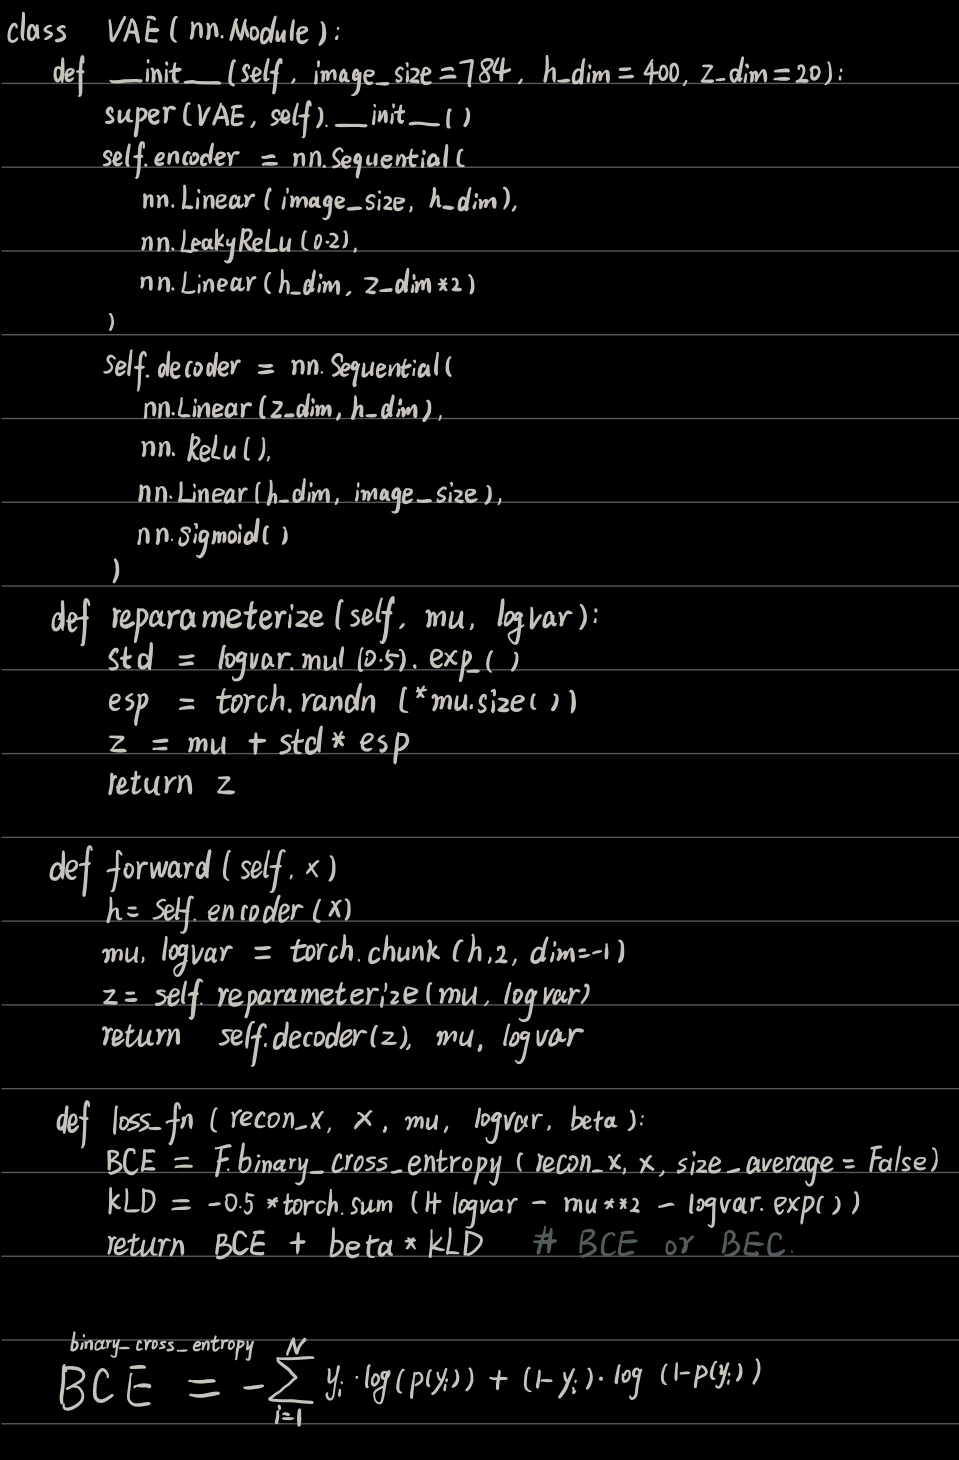
\includegraphics[width=0.9\linewidth]{figures/002.jpg}
    \caption{{\small 变分自编码器基本版的代码实现}}
    \label{fig:002}
\end{figure}
    图\ref{fig:002} 是一个对图片分类的简单的VAE的pytorch实现。输入的形式可以使图片也可以是词向量,所以这里以图片分类为例介绍不会影响对ETM模型的理解有影响
    并且以图片为例进行解释更加直观。
    
    初始化时构建了整个神经网络构架,一个编码器和一个与之对应的解码器。我们首先会把我们的图片通过编码器压缩到隐空间,在因空间中的图片信息会最大程度的保留。然后我们可以通过
    解码器把隐空间的数据解码成我们原来直观的图片形式。因此,编码器的输入和解码器的输出具有相同的维度。为了防止过拟合,我们假设我们编码后的信息不是一个点,而是一个分布,
    我们把这个分布假设成高斯分布——最完美的分布。我们通过解码器得到的是这个分布的均值和方差,从而得到了这个图片的分布,我们在这个分布上进行采样(代码中对应reparameterize类函数)
    越靠近分布中心的样本解码出来和原图就越相似。相应的主题模型中,我们提取一片文档的主题是,就只会在分布中心进行采样得到文档最有信息价值的话题。我们可以运用这些信息进行分类,
    判断文本的相似度。
    
    从图\ref{fig:002} 中我们可以看出损失函数包含两部分,但是和我们个公式\eqref{eq:002} 不是很相似,因为这其中是使用了一些技巧和变化的。
    这两部分也是我们上文提到的模型参数的损失值和变分参数的损失值。下面我们会介绍代码中的损失值是如何得来的。
\subsubsection{VAE损失函数的由来}
    首先,自编码器是有损的压缩,我么只能通过不断地训练模型来减小压缩损失。先假设我们有一个理想的编码器$ p(z|x) $,一个理想的解码器$ p(x|z) $和一个隐变量完美分布$ p(z) $。
    在这三个函数下我们能将任意一张图片$ x $压缩,得到隐变量Z。根据分布$ p(z) $得到解码器$p(x|z) $的输入,最后得到原来的图片$ x $而没有任何的损失。但是,我们不知道如何才能得到
    这样三个分布。在变分自编码器中,我们用“万能的”神经网络去无限逼近这些函数。编码器逼近$ p(z|x) $,解码器逼近$ p(x|z) $,对于隐变量我们给出了他的一个先验分布,假设$ p(z) $是一个高斯分布,
    可能实际上并不是高斯分布,我们只能用这个先验分布去无限逼近这个实际中的分布。总之,在训练的过程中我们需要不断逼近这个先验分布,尽管它可能符合实际的分布不是高斯分布的类型。
    
    假设我们编码器对应的分布为$ q(x|z) $, 我们需要在训练的过程中使$ q(x|z) $不断逼近$ p(x|z) $。上面我们介绍到了,$ \mathcal{KL} $散度是判断两个分布相似与否的评价标准。
    那么我们的损失函数就可以表示为:
\begin{equation}
    \begin{aligned}
        Loss &= \mathcal{KL}(q(x|z), p(x|z)) \\
        &= H(q(x|z), p(x|z)) - H(p(x|z)).
    \end{aligned}
    \label{eq:006}
\end{equation}
    那么降低Loss 可以从两方面入手: $ H(q,p) $ 越小越好,$  H(q)  $越大越好。    
    如果对于某张图片的编码长得像一个熵很大的高斯,那我们就不用担心$  H(q)  $很小,只要能好好套住它,这张图片的 Loss 也能降到 0;
    如果对于某张图片的编码分布长得不像高斯,那我们也没法硬套,只好让 $ H(q) $ 大点,也就是我们的高斯扁平一些,来尽可能地近似最优的编码分布。
    
    可是,我们并不知道$ p(z|x) $,我们又怎么能计算这个损失函数Loss呢?由公式\eqref{eq:003}\eqref{eq:004}\eqref{eq:005}得出下面的推导过程,如公式\eqref{eq:007}所示。
\begin{strip}
\begin{equation}
    \begin{aligned}
        Loss &= \mathcal{KL}(q(x|z), p(x|z)) \\
            &= H(q(x|z), p(x|z)) - H(p(x|z)) \\
            &= \left[ -\mathbb{E}_{q(z|x)}(\log \frac{p(z)\cdot p(x|z)}{p(x)}) \right] - \left[ -\mathbb{E}_{q(z|x)}(\log q(z|x)) \right] \\
            &= - \mathbb{E}_{q(z|x)}(\log p(x|z)) + \mathbb{E}_{q(z|x)}(\log p(x)) + \mathbb{E}_{q(z|x)}(\log q(z|x)) - \mathbb{E}_{q(z|x)}(\log p(z))\\
            &= - \mathbb{E}_{q(z|x)}(\log p(x|z)) + \log p(x) + \mathcal{KL}(q(z|x), p(z)) \\
            &= - \mathbb{E}_{q(z|x)}(\log p(x|z)) + \mathcal{KL}(q(z|x), p(z)) \\
            &= - \mathbb{E}_{q(z|x)}(\frac{\lVert x-f(z) \rVert^2}{2c}) + \mathcal{KL}(q(z|x), p(z)).
    \end{aligned}    
    \label{eq:007}
\end{equation}

\begin{equation}
    \begin{aligned}
        \mathcal{KL}(q(z|x), p(z)) &= \int \frac{1}{\sqrt{2\pi\sigma_q^2}}\exp\left( -\frac{(z-\mu_q)^2}{2\sigma_q^2} \right)   \log\left( \frac{ \frac{1}{\sqrt{2\pi\sigma_p^2}}\exp\left( -\frac{(z-\mu_p)^2}{2\sigma_p^2} \right) }{ \frac{1}{\sqrt{2\pi\sigma_q^2}}\exp\left( -\frac{(z-\mu_q)^2}{2\sigma_q^2} \right) }\right) dz \\
        &= \int \frac{1}{\sqrt{2\pi\sigma_q^2}}\exp\left( -\frac{(z-\mu_q)^2}{2\sigma_q^2} \right)\times \left(-\frac{1}{2}\log2\pi\sigma_p^2 - \frac{(z-\mu_p)^2}{2\sigma_p^2}  + \frac{1}{2}\log2\pi\sigma_q^2 + \frac{(z-\mu_q)^2}{2\sigma_q^2}  \right)dz\\
        &= \int \frac{1}{\sqrt{2\pi\sigma_q^2}}\exp\left( -\frac{(z-\mu_q)^2}{2\sigma_q^2} \right)\times \left(\log\frac{\sigma_p}{\sigma_p} - \frac{(z-\mu_p)^2}{2\sigma_p^2}  +  \frac{(z-\mu_q)^2}{2\sigma_q^2}  \right)dz\\
        &= \mathbb{E}_q\left\{ \log\frac{\sigma_p}{\sigma_p} - \frac{(z-\mu_p)^2}{2\sigma_p^2}  +  \frac{(z-\mu_q)^2}{2\sigma_q^2} \right\} \\
        &= \log\frac{\sigma_q}{\sigma_p} - \mathbb{E}_q\left\{  \frac{(z-\mu_p)^2}{2\sigma_p^2} \right\}  +   \mathbb{E}_q\left\{  \frac{(z-\mu_q)^2}{2\sigma_q^2} \right\} \\
        &= \log\frac{\sigma_q}{\sigma_p} - \frac{1}{2\sigma_p^2} \mathbb{E}_q\left\{ (z-\mu_p)^2 \right\}  +  \frac{1}{2} \\
        &= \log\frac{\sigma_q}{\sigma_p} - \frac{1}{2\sigma_p^2} \mathbb{E}_q\left\{ (z-\mu_q+ \mu_q-\mu_p)^2 \right\}  +  \frac{1}{2} \\
        &= \log\frac{\sigma_q}{\sigma_p} - \frac{1}{2\sigma_p^2} \mathbb{E}_q\left\{ (z-\mu_q)^2 +2(z-\mu_q)(\mu_q-\mu_p) + (\mu_q-\mu_p)^2 \right\}  +  \frac{1}{2} \\
        &= \log\frac{\sigma_q}{\sigma_p} - \frac{1}{2\sigma_p^2} \left[ \sigma_q^2 +2*0*(\mu_q-\mu_p) + (\mu_q-\mu_p)^2 \right]  +  \frac{1}{2} \\
        &= \log\sigma_q - \frac{ \sigma_q^2 + (\mu_q-\mu_p)^2 }{2\sigma_p^2}  +  \frac{1}{2} \\
        &= \log\sigma_q - \frac{ \sigma_q^2 + \mu_q^2 }{2}  +  \frac{1}{2} \\
        &= \frac{1}{2}\left( \log\sigma_q^2  +  1 - \sigma_q^2 - \mu_q^2  \right).
    \end{aligned}
    \label{eq:008}
\end{equation}
\end{strip}
    在公式\eqref{eq:007}的倒数第二行我们省略了$ \log p(x) $,是因为他是一个常数对我们训练时求梯度没有任何影响,去掉它不会影响最后参数的优化。
    在最终的结果中$ f(z) $表示解码器对$ z $进行解码,得到神经网络的输出$ \hat{x} $。$c$ 是一个超参数,当我们$ c $设置的比较小的时候,表示我们
    更愿意相信手里的数据集;当我们$ c $设置的比较大的时候,表示我们更愿意相信我们选择的先验分布。
    
    到此我们就得到了损失函数的一半,下面我们计算$ \mathcal{KL}(q(z|x), p(z)) $。
    首先,$ p(z) $和$ q(z|x) $是先验分布,分别表示为:
\begin{equation}
    p(z) = \frac{1}{\sqrt{2\pi\sigma_p^2}}\exp\left( -\frac{(z-\mu_p)^2}{2\sigma_p^2} \right)
    \label{eq:009}
\end{equation}
\begin{equation}
    q(z|x) = \frac{1}{\sqrt{2\pi\sigma_q^2}}\exp\left( -\frac{(z-\mu_q)^2}{2\sigma_q^2} \right)
    \label{eq:010}
\end{equation}
    其中,$ \mu_p,\sigma_p $是先验分布的参数,实常数;,$ \mu_q,\sigma_q $是的编码器的算出来的,在单个样本的Loss
    计算中也是常数。
    
    得到这些后我们算出Loss函数的后一部分,如公式\eqref{eq:008}。最后求出来的结果就是Loss的损失函数的后面一半。公式\eqref{eq:007}和公式\eqref{eq:008}
    就是最后损失函数:
\begin{equation}
    \begin{aligned}
        Loss =& - \mathbb{E}_{q(z|x)}(\frac{\lVert x-f(z) \rVert^2}{2c}) \\
              & + \frac{1}{2}\left( \log\sigma_q^2  +  1 - \sigma_q^2 - \mu_q^2  \right).
    \end{aligned}
    \label{eq:011}
\end{equation}
    这和图\ref{fig:002} 中损失函数的代码相一致。
    
    总之,通过神经网络和一些技巧,我们就可以无限逼近最优的$ p(z|x), p(x|z), p(z) $,得到训练好的参数。
\section{代码实践}
    在代码实现部分,我们使用的配置是:Windows,Python,pytorch。由于硬件设备比较差的原因,我们也没有使用比较的是聚集,训练的轮次也只有100轮。模型的具体实现详见附件。
\subsection{数据及介绍与预处理}
    数据集来源是《三体》第一部全书的内容,下图\ref{fig:003}给出了文章的一些文字片段。
\begin{figure}
    \centering
    
\includegraphics[width=0.9\linewidth]{figures/003}
    \caption{{\small《三体》第一步文章片段展示}}
    \label{fig:003}
\end{figure}
    对于中文文本我们需要一个分词器把没有空格的分开的句子分隔开。而在训练过程中标点符号和特殊符号是不可训练的,我们
    需要特殊处理和清除。
    我们使用的分词包是$ pyhanlp $, 它不仅能分词,而且能标记出分词后各个词的属性。如下代码所示:
\begin{minted}{python}
from pyhanlp import *
out = HanLP.segment('我来自电子科技大学。')
str(out)
Out[15]: '[我/rr, 来自/v, 电子科技大学/ntu, 。/w]'
\end{minted}
    经过分词器处理之后,我们的文本就像英文一样,单词和单词之间会有空格隔开。
\begin{minted}{python}
def tokenize(self, lines: List[str]) -> List[List[str]]:
    docs = []
    for line in tqdm(lines):
        tokens = [t.word for t in 
                    HanLP.segment(line)]
        tokens = [re.sub(self.pat, r'', t).strip() 
                    for t in tokens]
        tokens = [t for t in tokens if t != '']
        if self.stopwords is not None:
            tokens = [t for t in tokens 
                    if not (t in self.stopwords)]
        docs.append(tokens)
    return docs
\end{minted}

    分词之后,我们把文本集放入一个词袋,并生成一个该文本集对应的字典。然后再统计单词出现的频率,对那些出现频率极低和出现频率极高的单词进行去除。把剩下的词汇给好编号以及单词的频率放入一个专门的类中。然后将词袋放入词向量编码模型得到每个词的词向量。得到词向量之后就可以直接放入变分自编码器中进行训练了。
    
    我们的参数设置:学习率0.005;参数优化器Adam; 词频低于3的次我们会剔除,单次出现率占0.5\%我们也会剔除;提取文本的最有可能的话题数20个;batch size设为512;使用CPU训练。参数详情如下:
\begin{minted}{python}
parser = argparse.ArgumentParser('ETM topic model')

parser.add_argument('--taskname', type=str, default='3body1',
help='Taskname e.g cnews10k')

parser.add_argument('--no_below', type=int, default=5,
help='The lower bound of count for words to keep, e.g 10')

parser.add_argument('--no_above', type=float, default=0.005,
help='The ratio of upper bound of count for words to keep')

parser.add_argument('--num_epochs', type=int, default=100,
help='Number of iterations (1000+ is recommended.)')

parser.add_argument('--n_topic', type=int, default=20,
help='Num of topics')

parser.add_argument('--bkpt_continue', type=bool, 
default=False, help='Whether to load a trained model as
initialization and continue training.')

parser.add_argument('--use_tfidf', type=bool, default=False,
help='Whether to use the tfidf feature for the BOW input')

parser.add_argument('--rebuild', type=bool, default=True,
help='Whether to rebuild the corpus, such as tokenization, 
build dict etc.(default True)')

parser.add_argument('--batch_size', type=int, default=512,
help='Batch size (default=512)')

parser.add_argument('--criterion',type=str,default=
'cross_entropy',help='The criterion to calculate the loss')

parser.add_argument('--emb_dim', type=int, default=300,
help="The dimension of the latent topic vectors")

parser.add_argument('--auto_adj', action='store_true',
help='To adjust the no_above ratio automatically')

parser.add_argument('--ckpt', type=str, default='',
help='Checkpoint path')

parser.add_argument('--lang', type=str, default="zh",
help='Language of the dataset')
\end{minted}

\subsection{结果展示}
    首先展示搭建的神经网络模型代码,分为两部分:1)变分自编码器代码,
\begin{minted}{python}
super(VAE, self).__init__()
self.encoder = nn.ModuleDict({
    f'enc_{i}': nn.Linear(encode_dims[i], encode_dims[i + 1])
    for i in range(len(encode_dims) - 2)
})
self.fc_mu = nn.Linear(encode_dims[-2], encode_dims[-1])
self.fc_logvar = nn.Linear(encode_dims[-2], encode_dims[-1])

self.decoder = nn.ModuleDict({
    f'dec_{i}': nn.Linear(decode_dims[i], decode_dims[i + 1])
    for i in range(len(decode_dims) - 1)
})
self.latent_dim = encode_dims[-1]
self.dropout = nn.Dropout(p=dropout)
self.fc1 = nn.Linear(encode_dims[-1], encode_dims[-1])
\end{minted}
    这里只给出了神经网络中的主要模块,编码解码过程请看附件。
    
    2)ETM模型框架代码,
\begin{minted}{python}
class EVAE(VAE):
    def __init__(self, encode_dims=[2000, 1024, 512, 20], 
                        decode_dims=[20, 1024, 2000], 
                        dropout=0.0, emb_dim=300):
        super(EVAE, self).__init__(encode_dims=encode_dims,
                    decode_dims=decode_dims, dropout=dropout)
        self.emb_dim = emb_dim
        self.vocab_size = encode_dims[0]
        self.n_topic = encode_dims[-1]
        self.rho = nn.Linear(emb_dim, self.vocab_size)
        self.alpha = nn.Linear(emb_dim, self.n_topic)
        self.decoder = None

    def decode(self, z):
        wght_dec = self.alpha(self.rho.weight)  # [K,V]
        beta = F.softmax(wght_dec, dim=0).transpose(1, 0)
        res = torch.mm(z, beta)
        logits = torch.log(res + 1e-6)
        return logits


class ETM:
    def __init__(self, bow_dim=10000, 
                        n_topic=20, 
                        taskname=None, 
                        device=None, 
                        emb_dim=300):
        self.bow_dim = bow_dim
        self.n_topic = n_topic
        self.emb_dim = emb_dim
        # TBD_fc1
        self.vae = EVAE(encode_dims=[bow_dim, 1024, 512, n_topic],
                        decode_dims=[n_topic, 512, bow_dim], 
                        dropout=0.0,
        emb_dim=emb_dim)
        self.device = device
        self.id2token = None
        self.taskname = taskname
        if device != None:
        self.vae = self.vae.to(device)
\end{minted}
	
	经过训练后我们的到训练过程中损失值的变化趋势如图\ref{fig:004} 所示。
\begin{figure}
	\centering
	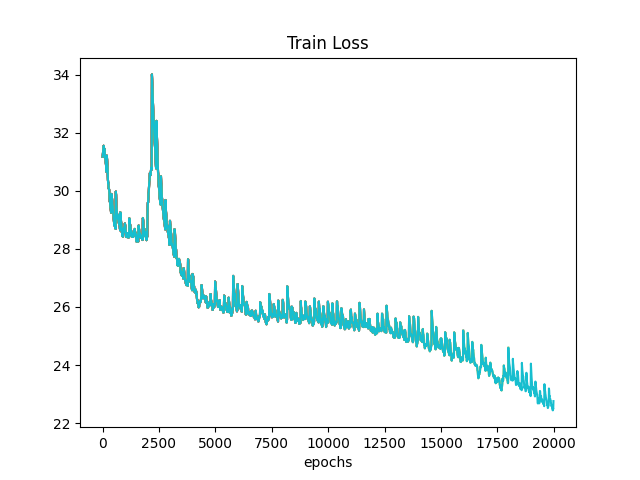
\includegraphics[width=0.9\linewidth]{figures/004.png}
	\caption{{\small 随着训练次数的增加,模型的损失值在不断地减小}}
	\label{fig:004}
\end{figure}

	经过训练后得到的主题如下图\ref{fig:005}所示,每个文档会得到20个话题,并且含有其相应的话题向量方便进一步的自然语言任务的处理。
\begin{figure}
	\centering
	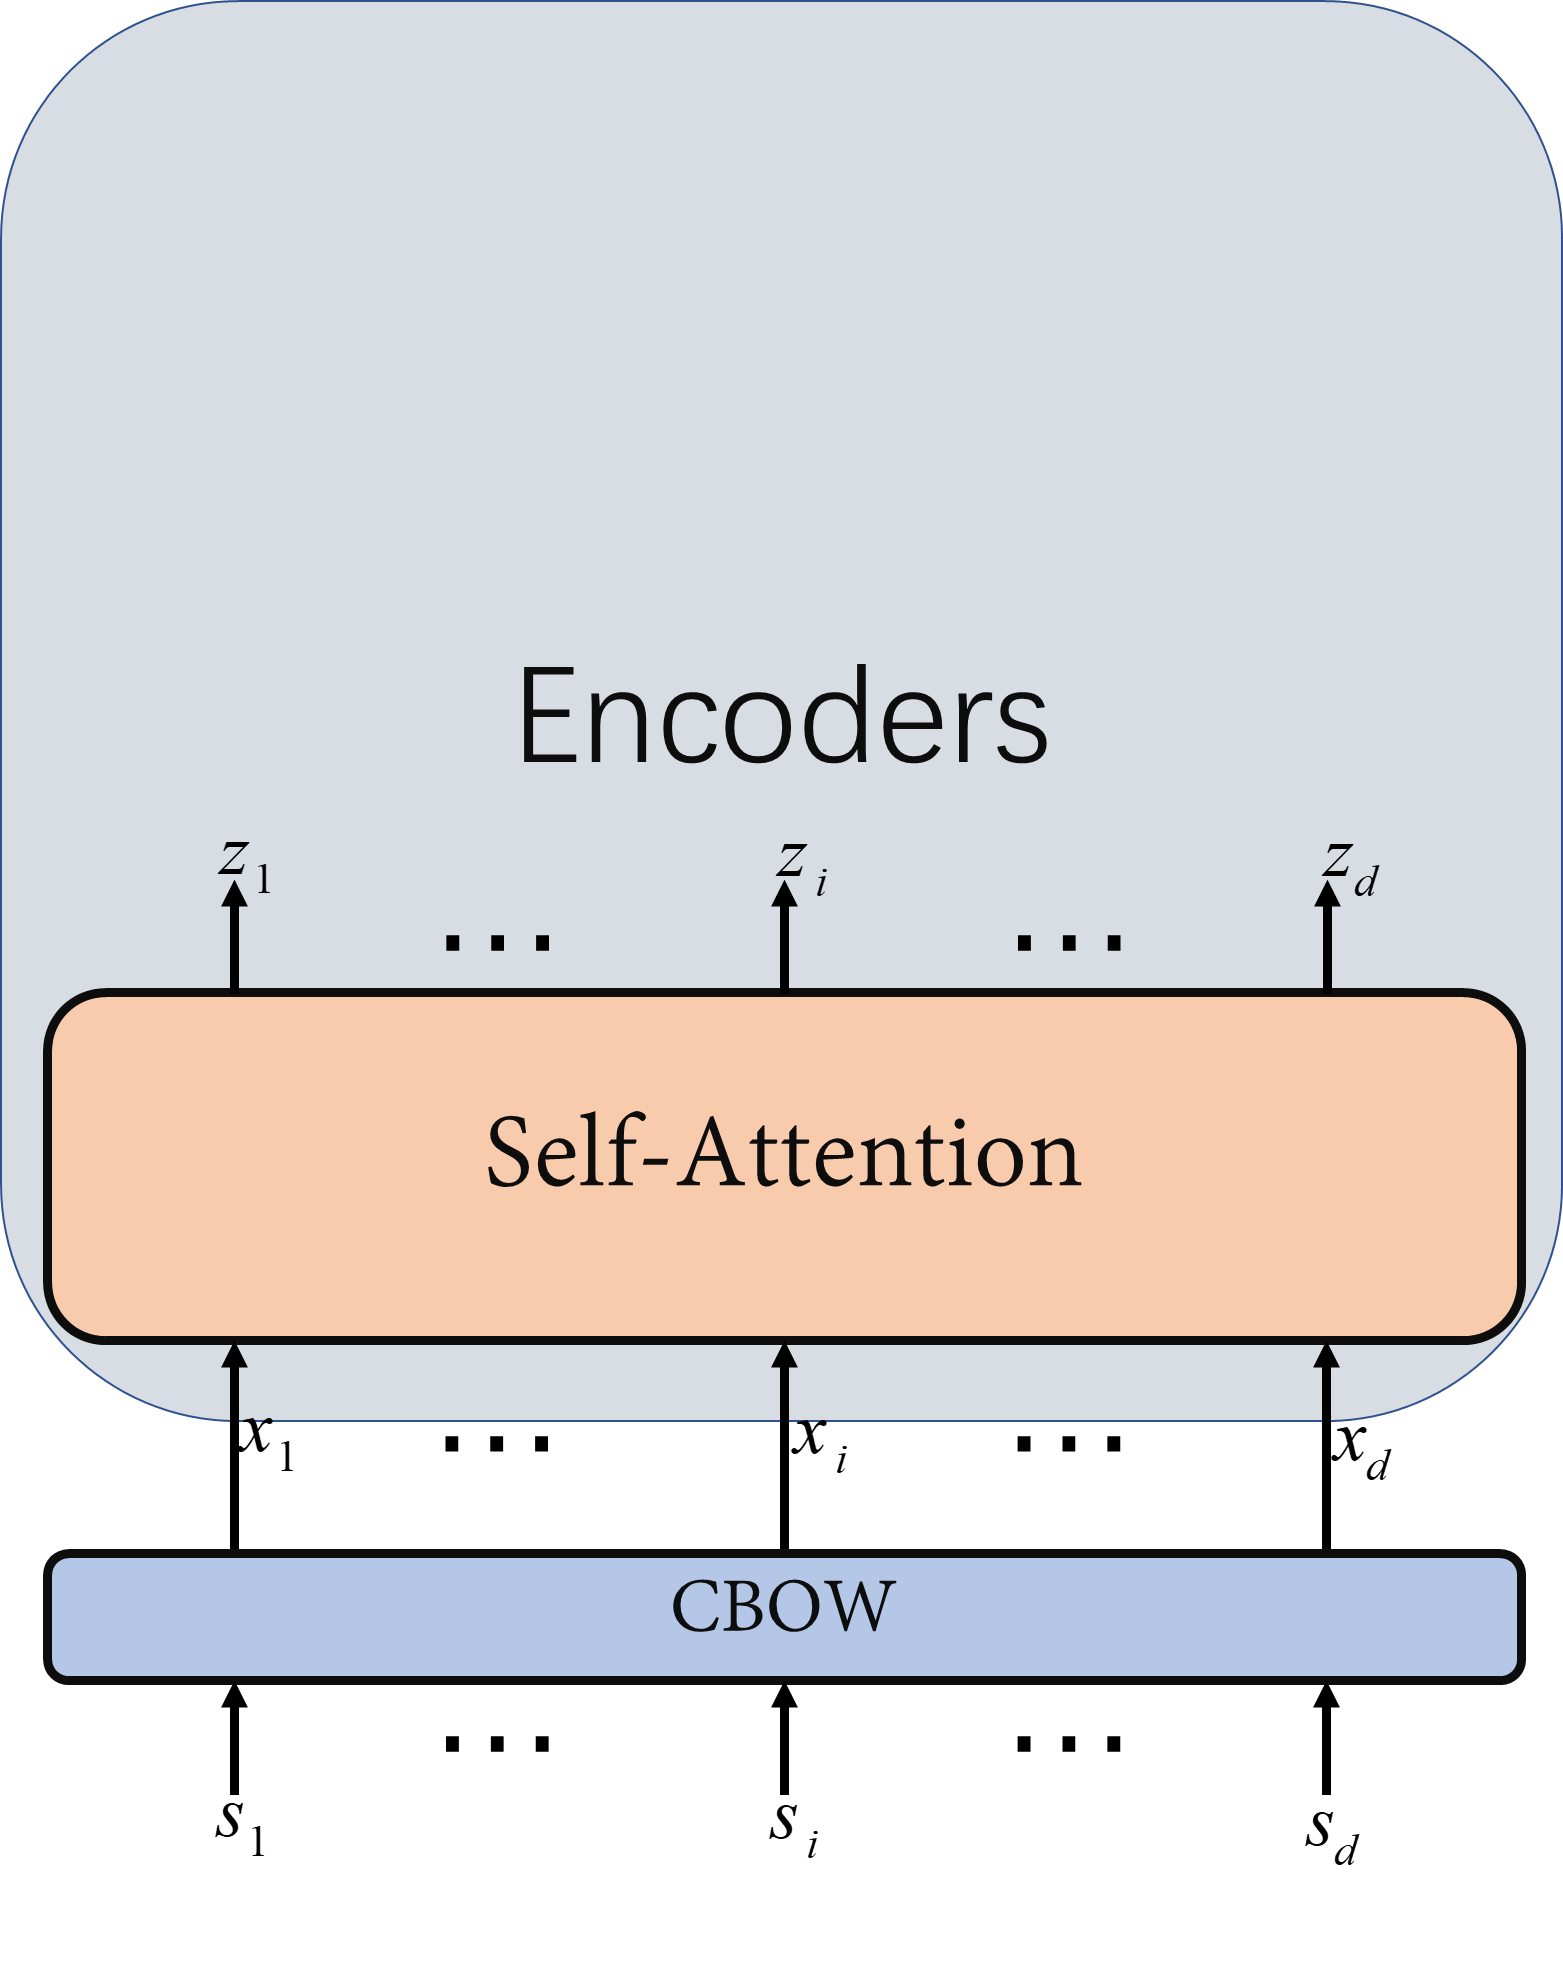
\includegraphics[width=0.9\linewidth]{figures/006.png}
	\caption{{\small 前10个文档在训练后得到的主题}}
	\label{fig:005}
\end{figure}
	
	由于是半监督训练,没有测试集。在得到主体后有,我们通过一些评测标准来判定一个文档话题与话题之间的连贯性和差异性。一般而言连贯性越好差异性越大,主题模型的效果越好。如图\ref{fig:006} 所示,是文档生成主题的两关系随着训练次数的增加而发生的变化。
\begin{figure}
	\centering
	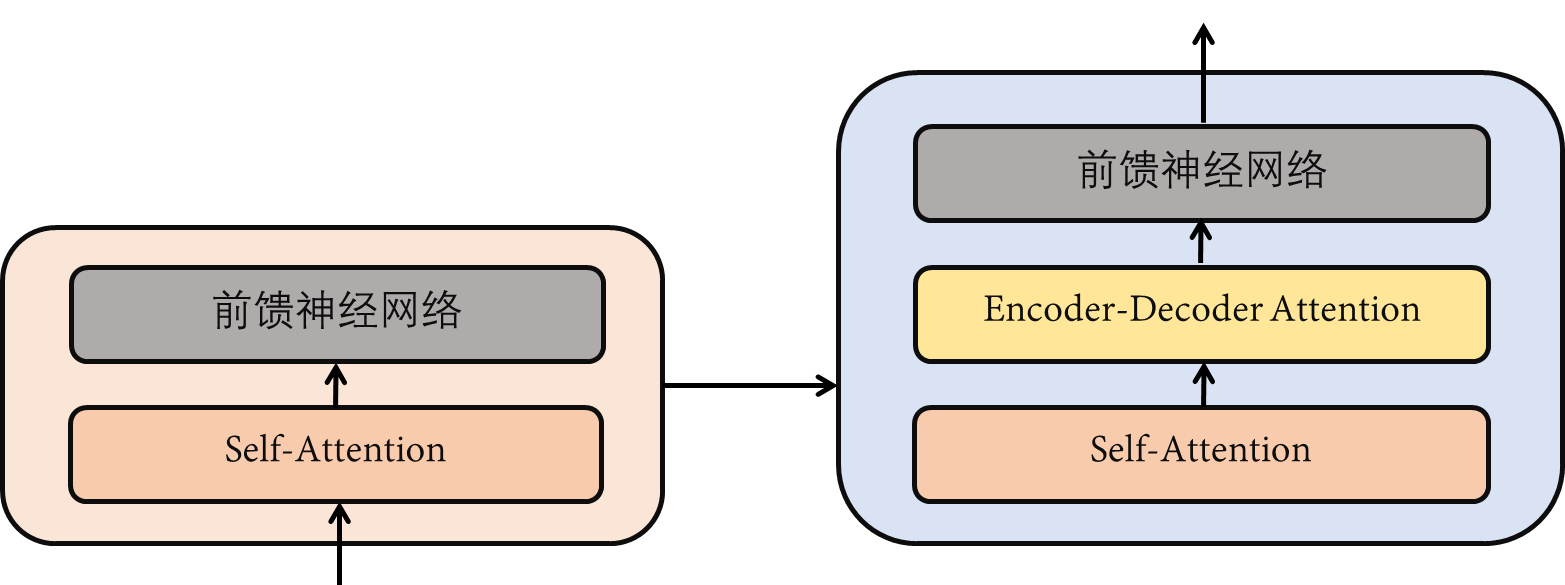
\includegraphics[width=0.9\linewidth]{figures/005.png}
	\caption{{\small 前10个文档在训练后得到的主题}}
	\label{fig:006}
\end{figure}	

\section{收获感受}
	经过本次论文的复现的学习,深刻了解到了主题模型的用处和用法,这对后面进行混合模型的文本分类任务打下了基础。
	同时也报聋了我的很多问题,数学方面的的基础较差。在面对一些概率模型的时候,还不能做一些灵活的转化,最后通过找资料才补回来。
	这篇论文只是在大致上浮现出来了,而实验中的很多细节我还是没有照顾到,在后面会进一步的完善。在了解到主题模型这个大家族后,
	也有了一些感触和想法,之后可能会结合词向量模型进行一些测试和验证。比较一下各个模型的效果,同时也去寻找一些多特征提取的混合
	模型。在得到文本不同角度特征后,看看能产生什么样的效果。

% 添加参考文献
\bibliographystyle{IEEEtran}    % 设置文献样式
\bibliography{sougoul.bib}    % 设置文献的文件路径
%\end{multicols}  
\newpage
%\section*{附录1: python实现线性回归所用代码} \label{appendix1}
%\begin{minted}{python}
%import os
%def f():
%    print('hello world')
%\end{minted}

\end{document}


